% Options for packages loaded elsewhere
\PassOptionsToPackage{unicode}{hyperref}
\PassOptionsToPackage{hyphens}{url}
%
\documentclass[
]{article}
\usepackage{amsmath,amssymb}
\usepackage{lmodern}
\usepackage{iftex}
\ifPDFTeX
  \usepackage[T1]{fontenc}
  \usepackage[utf8]{inputenc}
  \usepackage{textcomp} % provide euro and other symbols
\else % if luatex or xetex
  \usepackage{unicode-math}
  \defaultfontfeatures{Scale=MatchLowercase}
  \defaultfontfeatures[\rmfamily]{Ligatures=TeX,Scale=1}
\fi
% Use upquote if available, for straight quotes in verbatim environments
\IfFileExists{upquote.sty}{\usepackage{upquote}}{}
\IfFileExists{microtype.sty}{% use microtype if available
  \usepackage[]{microtype}
  \UseMicrotypeSet[protrusion]{basicmath} % disable protrusion for tt fonts
}{}
\makeatletter
\@ifundefined{KOMAClassName}{% if non-KOMA class
  \IfFileExists{parskip.sty}{%
    \usepackage{parskip}
  }{% else
    \setlength{\parindent}{0pt}
    \setlength{\parskip}{6pt plus 2pt minus 1pt}}
}{% if KOMA class
  \KOMAoptions{parskip=half}}
\makeatother
\usepackage{xcolor}
\IfFileExists{xurl.sty}{\usepackage{xurl}}{} % add URL line breaks if available
\IfFileExists{bookmark.sty}{\usepackage{bookmark}}{\usepackage{hyperref}}
\hypersetup{
  pdftitle={Day 1},
  hidelinks,
  pdfcreator={LaTeX via pandoc}}
\urlstyle{same} % disable monospaced font for URLs
\usepackage[margin=1in]{geometry}
\usepackage{longtable,booktabs,array}
\usepackage{calc} % for calculating minipage widths
% Correct order of tables after \paragraph or \subparagraph
\usepackage{etoolbox}
\makeatletter
\patchcmd\longtable{\par}{\if@noskipsec\mbox{}\fi\par}{}{}
\makeatother
% Allow footnotes in longtable head/foot
\IfFileExists{footnotehyper.sty}{\usepackage{footnotehyper}}{\usepackage{footnote}}
\makesavenoteenv{longtable}
\usepackage{graphicx}
\makeatletter
\def\maxwidth{\ifdim\Gin@nat@width>\linewidth\linewidth\else\Gin@nat@width\fi}
\def\maxheight{\ifdim\Gin@nat@height>\textheight\textheight\else\Gin@nat@height\fi}
\makeatother
% Scale images if necessary, so that they will not overflow the page
% margins by default, and it is still possible to overwrite the defaults
% using explicit options in \includegraphics[width, height, ...]{}
\setkeys{Gin}{width=\maxwidth,height=\maxheight,keepaspectratio}
% Set default figure placement to htbp
\makeatletter
\def\fps@figure{htbp}
\makeatother
\setlength{\emergencystretch}{3em} % prevent overfull lines
\providecommand{\tightlist}{%
  \setlength{\itemsep}{0pt}\setlength{\parskip}{0pt}}
\setcounter{secnumdepth}{-\maxdimen} % remove section numbering
\ifLuaTeX
  \usepackage{selnolig}  % disable illegal ligatures
\fi

\title{Day 1}
\usepackage{etoolbox}
\makeatletter
\providecommand{\subtitle}[1]{% add subtitle to \maketitle
  \apptocmd{\@title}{\par {\large #1 \par}}{}{}
}
\makeatother
\subtitle{Welcome to ISSSV1337}
\author{}
\date{\vspace{-2.5em}27. June 2022}

\begin{document}
\maketitle

Hello everyone!

Welcome to Political Data Science Hackathon. We're thrilled to have you
here with us, and we look forward to spending a great and interesting
summer together.

\hypertarget{what-is-a-hackathon}{%
\subsubsection{What is a hackathon?}\label{what-is-a-hackathon}}

Hackathons are a bit like festivals. People come together in an intense
and focused setting to have a shared experience. One of the main
differences, I would say, is that in a hackathon you also work together
in a team to create something. By definition, hackathons are events in
which ``a large number of people meet to engage in collaborative
computer programming.'' Usually, the end goal is to produce something,
like a game, a software, or an API.

Hackathons are great because they allow us to be reminded of a few
important facts: (1) Team-work is awesome when it works, (2) We can
create great things in short time if we work with focus and (3) One of
the best ways to learn is learning by doing.

Oh, and failing is a part of the process.

Naturally, we do not expect you to sit tight six weeks in a row and work
with iron focus on your tasks throughout the summer months. However, we
hope that you will take some of the ideas behind hackathons to heart.
This is a playground just as much as it is a course. Learning, creating
and producing is supposed to be challenging, rewarding, frustrating and
- especially - fun! We hope this course will allow you to experience
just that.

\hypertarget{how-does-this-course-work}{%
\subsubsection{How does this course
work?}\label{how-does-this-course-work}}

This course runs over six weeks. You will produce a report (or an app,
if you like), that is related to a problem statement. The problem
statements are provided by actors from work life. You work in teams with
people from different disciplinary backgrounds. In the end, you present
your final product to the rest of us and the work life actors, and one
team wins the hackathon. They receive a price! Otherwise, the course is
pass/fail.

Most days we provide some tasks to work on in the second half of the
lecture, but there are no hand-ins except for the final report. The
lectures run from 10:00 to 12:00, and are organized so that the first
hour is theory, while the second hour is focused on practice.

Please note: \emph{In the third week, we have a long weekend (14.-17.
June) and from week 4, we change location from Blindern to Statistics
Norway (Akersveien 26).}

\hfill\break

That was a little bit about the structure. Now, about the content.
Throughout the course, we have three goals in mind:

\begin{enumerate}
\def\labelenumi{\arabic{enumi}.}
\tightlist
\item
  Introduce and teach some basic data science skills.
\item
  Demonstrate how to work effectively in cross-disciplinary teams.
\item
  Give an opportunity to learn and produce something worklife related.
\end{enumerate}

This course will not cover everything data science related. In fact, it
will only give you a glimpse into the world of data science. However,
hopefully it will give you the knowledge you need to pursue more
knowledge. You see, data science is a highly cross-disciplinary field,
and we need people with different competences. To illustrate, look at
the figure below. Many would agree that data science is some sort of
cross-over between computer science, statistics and domain expertise.
Often, this means building high-end knowledge in one of the circles, and
knowing enough about the other circles to be able to work in team-based
contexts to draw on each other's specialties. Being able to understand,
translate and work cross-disciplinary is an incredibly useful skill.

\begin{figure}
\centering
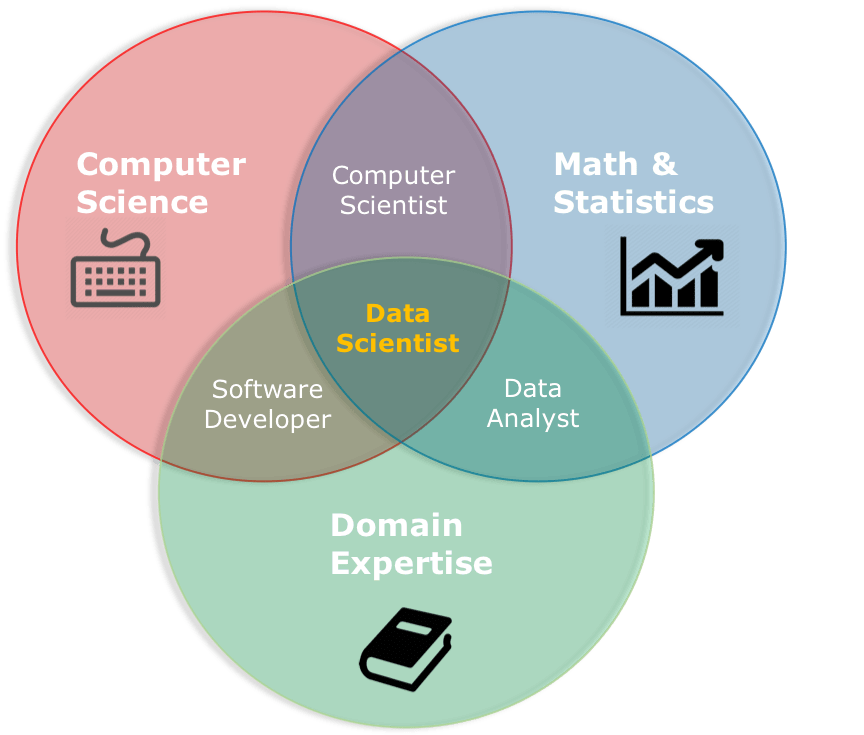
\includegraphics[width=0.5\textwidth,height=\textheight]{https://github.com/sbjorkholt/ISSSV1337/blob/main/Week\%201/scripts/figures/datascience_figure.png?raw=true}
\caption{The cross-disciplinary nature of data science.}
\end{figure}

So, what do we mean by the different points above? Well, in short:

\emph{1. Introduce and teach some basic data science skills.}

\begin{itemize}
\tightlist
\item
  Using R (functions, visualization, paths)
\item
  Collaborating using Github
\item
  Finding data (working with databases, APIs and webpages)
\item
  Programming with text
\item
  Machine learning (supervised and unsupervised)
\end{itemize}

\emph{2. Demonstrate how to work effectively in cross-disciplinary
teams.}

\begin{itemize}
\tightlist
\item
  Working under agile principles.
\item
  Using know-how from team-based work.
\end{itemize}

\emph{3. Give an opportunity to learn and produce something work life
related.}

\begin{itemize}
\tightlist
\item
  Work on a problem statement provided by work life organizations.
\item
  Get some examples on how data science can be used in work-life
  contexts.
\end{itemize}

Here is a table over what we will cover in each week:

\begin{longtable}[]{@{}
  >{\raggedright\arraybackslash}p{(\columnwidth - 10\tabcolsep) * \real{0.0571}}
  >{\raggedright\arraybackslash}p{(\columnwidth - 10\tabcolsep) * \real{0.0762}}
  >{\raggedright\arraybackslash}p{(\columnwidth - 10\tabcolsep) * \real{0.1048}}
  >{\raggedright\arraybackslash}p{(\columnwidth - 10\tabcolsep) * \real{0.0952}}
  >{\raggedright\arraybackslash}p{(\columnwidth - 10\tabcolsep) * \real{0.1238}}
  >{\raggedright\arraybackslash}p{(\columnwidth - 10\tabcolsep) * \real{0.5429}}@{}}
\toprule
\begin{minipage}[b]{\linewidth}\raggedright
Week
\end{minipage} & \begin{minipage}[b]{\linewidth}\raggedright
Date
\end{minipage} & \begin{minipage}[b]{\linewidth}\raggedright
Day
\end{minipage} & \begin{minipage}[b]{\linewidth}\raggedright
Location
\end{minipage} & \begin{minipage}[b]{\linewidth}\raggedright
Time
\end{minipage} & \begin{minipage}[b]{\linewidth}\raggedright
Topic
\end{minipage} \\
\midrule
\endhead
1 & 27.jun & Monday & Blindern & 10:15-12:00 & Introduction to course \\
1 & 28.jun & Tuesday & Blindern & 10:15-12:00 & Workflow \& Github \\
1 & 29.jun & Wednesday & Blindern & 10:15-12:00 & Introduction to data
analysis and data transformation \\
1 & 30.jun & Thursday & Blindern & 10:15-12:00 & Descriptive statistics
and relational data \\
1 & 01.jul & Friday & Blindern & 10:15-12:00 & Presentations from
stakeholders \\
2 & 04.jul & Monday & Blindern & 10:15-12:00 & Data sources \& SQL \\
2 & 05.jul & Tuesday & Blindern & 10:15-12:00 & Webscraping \\
2 & 06.jul & Wednesday & Blindern & 10:15-12:00 & API \\
2 & 07.jul & Thursday & Blindern & 10:15-12:00 & Data visualisation with
ggplot \\
2 & 08.jul & Friday & Blindern & 10:15-12:00 & Data visualisation with
plotly and Rmarkdown \\
3 & 11.jul & Monday & Blindern & 10:15-12:00 & Bag of words and
TF-IDF \\
3 & 12.jul & Tuesday & Blindern & 10:15-12:00 & N-grams, tidying and
plotting \\
3 & 13.jul & Wednesday & Blindern & 10:15-12:00 & Topic modelling \\
4 & 18.jul & Monday & SSB & 10:15-12:00 & Machine learning
introduction \\
4 & 19.jul & Tuesday & SSB & 10:15-12:00 & Models \\
4 & 20.jul & Wednesday & SSB & 10:15-12:00 & Supervised learning:
Regression \\
4 & 21.jul & Thursday & SSB & 10:15-12:00 & Supervised learning:
Classification \\
4 & 22.jul & Friday & SSB & 10:15-12:00 & Loss functions \\
5 & 25.jul & Monday & SSB & 10:15-12:00 & Unsupervised learning \\
5 & 26.jul & Tuesday & SSB & 10:15-12:00 & Text and machine learning \\
5 & 27.jul & Wednesday & SSB & 10:15-12:00 & Deployment \& iterative
work \\
5 & 28.jul & Thursday & SSB & 10:15-12:00 & IT knowledge \\
5 & 29.jul & Friday & SSB & 10:15-12:00 & Open day \\
6 & 01.aug & Monday & SSB & 10:15-12:00 & Case presentation \\
6 & 02.aug & Tuesday & SSB & 10:15-12:00 & Case presentation \\
6 & 03.aug & Wednesday & SSB & 10:15-12:00 & Case presentation \\
6 & 04.aug & Thursday & SSB & 10:15-12:00 & Final presentations \\
\bottomrule
\end{longtable}

\hypertarget{what-do-we-expect-from-you}{%
\subsubsection{What do we expect from
you?}\label{what-do-we-expect-from-you}}

\textbf{Attendance}: We would like you to show up to every session.
Formally, you must attend a minimum of 75\% of the lectures in order to
take the final exam (i.e.~participate in the presentations in the end
and get a pass/fail assessment).

\textbf{Team work}: We expect that you work together with your team
members on the problem statement. You can decide yourselves how you
would like to work, but we recommend meeting physically at least two
times a week for a session of 2-4 hours. This makes it easier to track
progress and it often makes working more rewarding. It is also useful to
set up a Teams, Slack or other communication channel. Keep in mind that
you may be on different levels with regard to programming skills, and
you may come from very different backgrounds. Try to utilize this rather
than view it as a hindrance. We reward teams that work to make each
other better - both in terms of programming skills and other skills.

Most importantly, for this to feel like an exciting but safe learning
space, we expect fun competitiveness and warm cooperativeness.

\hypertarget{how-and-why-to-work-agile}{%
\subsubsection{How and why to work
agile?}\label{how-and-why-to-work-agile}}

\hypertarget{the-belbin-strength-test}{%
\subsubsection{The Belbin Strength
test}\label{the-belbin-strength-test}}

\hypertarget{links}{%
\subsubsection{Links}\label{links}}

Should you wish to participate in some hackathons, here is a list of
some events:

\end{document}
